\chapter{Using the QPU Directly}\label{sec:qpuonly}

\section{Analysis of Hybrid Solving Times}

Section \ref{sec:qsvm-res} has shown that adiabatic quantum computing can offer advantages in terms of faster convergence to a solution. However, it is worth asking how much of this advantage is due to the quantum component and how much is attributable to a classical solver optimised for quadratic problems.

The technology behind the hybrid solvers is protected by D-Wave's intellectual property, which makes these tools essentially black boxes. Given the proprietary nature of these solvers, analysis must rely on the limited data available to make informed evaluations of alternative solutions.
From the control dashboard provided by D-Wave\footnote{\url{https://cloud.dwavesys.com/leap/}}, it is possible to inspect the problems solved by their QPUs and obtain some useful information.

Although the data collected does not allow an in-depth analysis of the underlying implementation choices, it can still be useful for a ``high-level'' analysis.
\begin{figure}
    \centering
    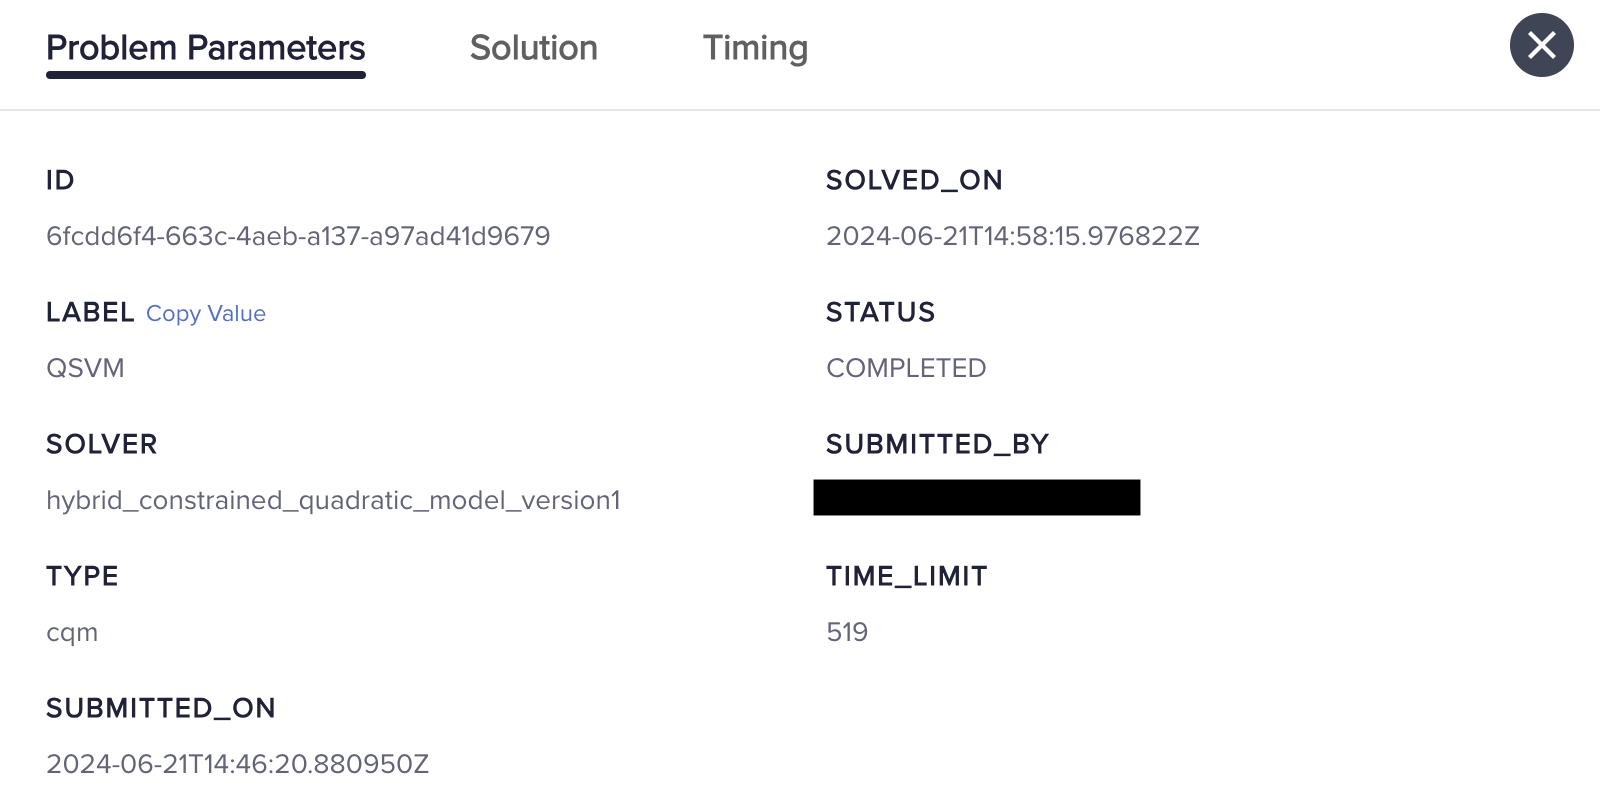
\includegraphics[width=0.8\textwidth]{figures/dashboard.png}
    \caption{D-Wave Leap dashboard.}
    \label{fig:dwaveleap}
\end{figure}
By selecting a problem from the list, the information from Figure \ref{fig:dwaveleap} is available, i.e: 
\begin{itemize} 
	\item A report on the characteristics of the problem presented, whether BQM, QUBO or CQM. 
	\item A list of the calculated potential solutions, together with the associated energy values, representing the result of the objective function with the given assignment, Figure \ref{fig:sampleset} is an example. 
	\item Execution times of the problem, indicating not only the total time but also how much of this time was spent on the QPU. 
\end{itemize}

\begin{figure}
    \centering
    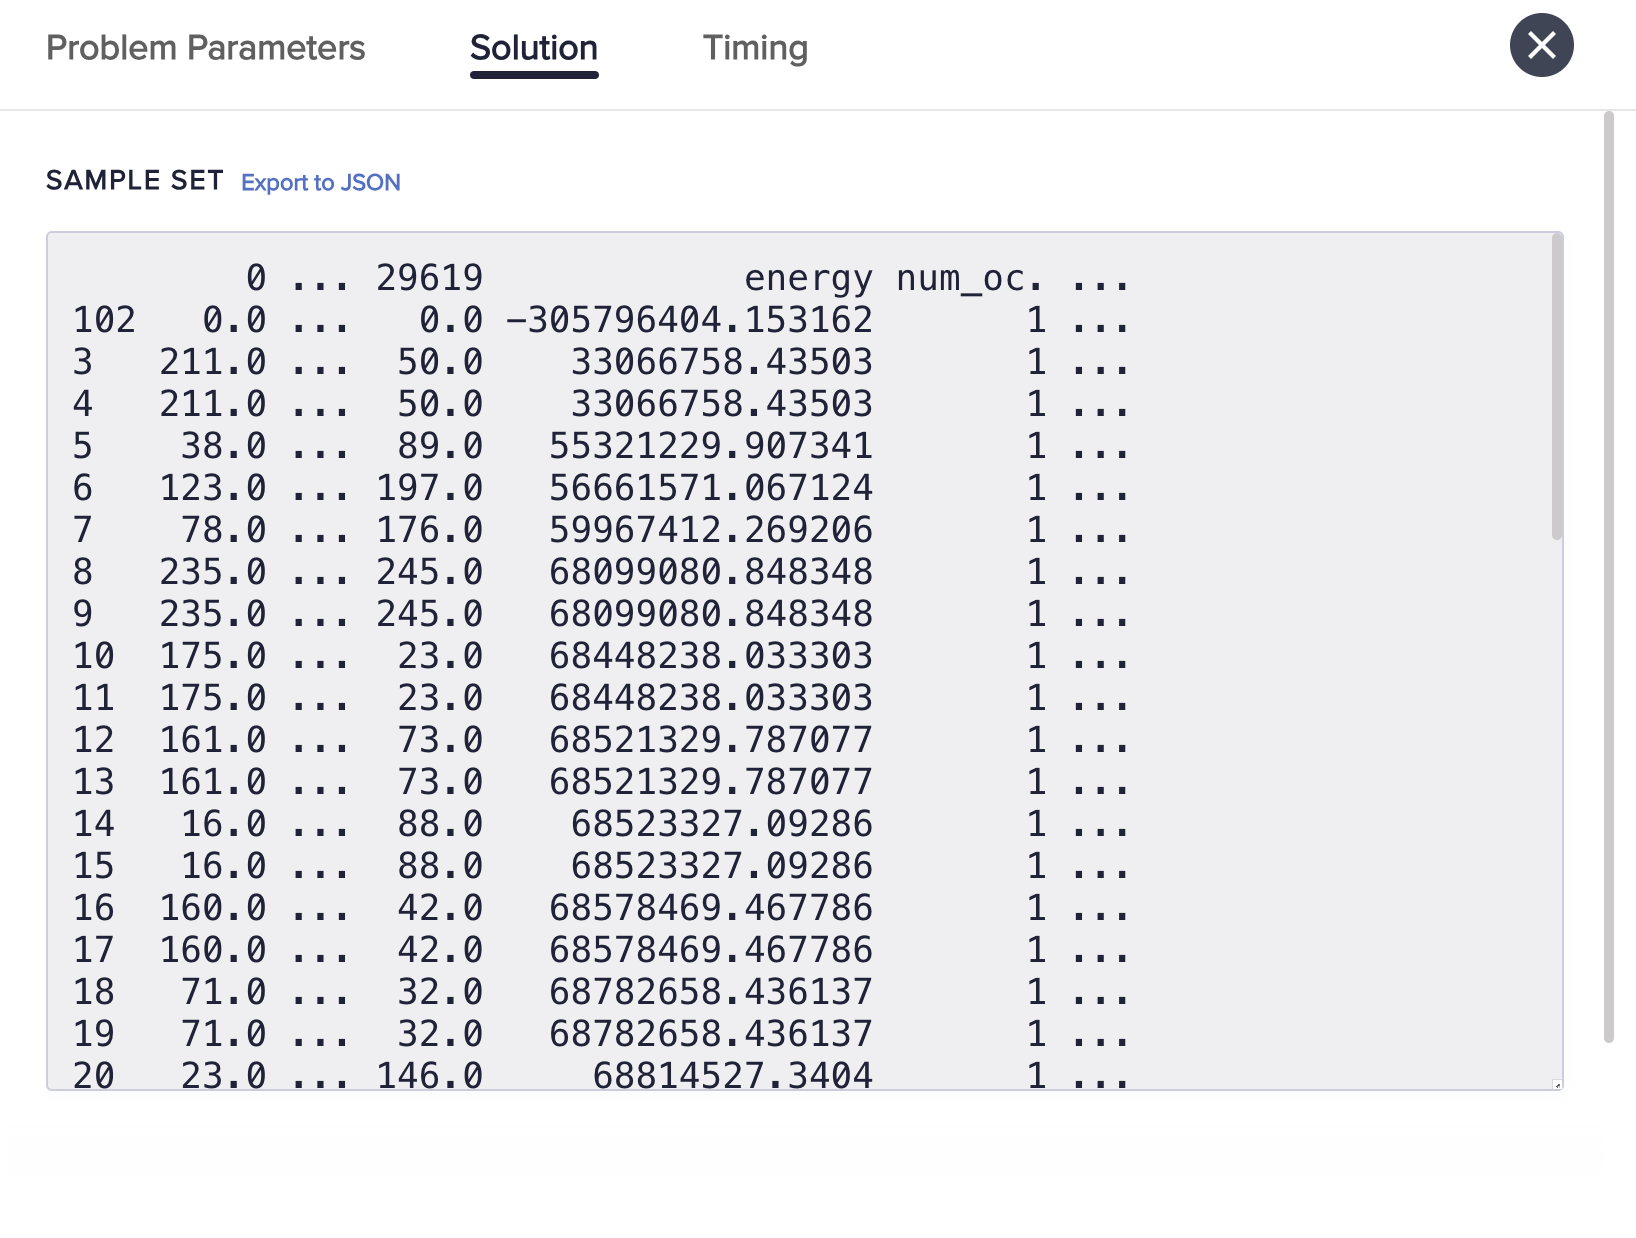
\includegraphics[width=0.8\textwidth]{figures/sampleset.png}
    \caption{List of solutions.}
    \label{fig:sampleset}
\end{figure}

Of the available data, information on execution times is of main interest, as it can help to determine whether and to what extent the quantum component is crucial in generating an optimal solution.

\subsection{QPU Usage}

Analysing the execution of the quantum support vector machine on a subset of TweetDF, it can be seen that of the 40 seconds it took to find the optimal solution, only 0.031 seconds were used by the QPU. Proportionally, the QPU was used for only 0.08\% of the total time required by the solver.

When using the entire TweetDF, the data indicated a QPU utilisation of 0.05 seconds, compared to the 480 seconds it took the solver to find a solution, reducing the QPU utilisation to 0.01\%.

These results highlight two fundamental aspects: 
\begin{itemize} 
	\item The use of the QPU is minimal compared to the classical component required to calculate the solution; 
	\item The use of the QPU seems to decrease as the problem size increases, while the time used by the classical component increases significantly. 
\end{itemize}

Considering that the D-Wave hybrid solver has proven to be more efficient than its classical counterpart, CPLEX, the question arises whether the performance improvement is due to the QPU or a superior classical solver.

As an alternative to D-Wave's hybrid approach, ``QPU-only'' solvers can be used. By manually performing the pre-processing steps, the classical reprocessing and resolution component can be avoided, while the entire calculation is performed on the QPU.

\paragraph{Free use of quantum solver} It is important to note that all observations made in this study pertain to behaviours recorded using the free tier of D-Wave's solvers. 
This plan offers 20 minutes per month for the hybrid solvers and one minute per month for purely quantum solvers.

It is not explicitly stated whether the paid plan involves using different algorithms compared to the free version. 
Given that, the free tier is presented as an opportunity for prototyping'', some of the findings gathered may not fully reflect the complete potential of the quantum technology provided by D-Wave.

\section{QPU solver}

The use of purely quantum solvers provided by D-Wave necessitates two main steps before a problem can be submitted to the QPU:

\begin{enumerate}
    \item Conversion of the problem into QUBO form;
    \item Transformation into an equivalent problem compatible with the QPU.
\end{enumerate}

As discussed in Section \ref{sec:dwaveconversion}, the former can be performed automatically using the libraries provided by D-Wave, which convert a problem expressed as an objective function and constraints (CSP) into an equivalent QUBO problem, i.e., $x^TQx$, as outlined in Section \ref{sec:AQC}.

The latter is related to minor embedding, which involves transforming the problem into an equivalent form that respects the qubit structure of the QPU.

The operations necessary to convert a CSP into a QUBO form can be executed in linear time. Therefore, if it were possible to perform minor embedding without requiring excessive computational resources or time, the use of the QPU without leveraging the hybrid component would present itself as a valid methodology for solving problems through adiabatic quantum computing.

The following sections will thus focus on analyzing the minor embedding algorithm, examining what has been implemented by D-Wave and the intrinsic complexity of the problem.

\section{Minor Embedding Algorithm}

\begin{displayquote}
    Given two arbitrary graphs $G$ and $H$, $G$ is called a minor of $H$ if $G$ is isomorphic to a graph that can be formed from $H$ by a series of the following operations: edge contraction, edge or vertex deletion.
\end{displayquote}

The definition provided introduces the concept of a minor graph, which is fundamental to understanding the applications of minor embedding. 

Recalling that two graphs are isomorphic if there exists a bijective function between the vertices of the first graph and those of the second.

In the minor embedding of $G$ into $H$, $G$ is the ``small'' graph that must be isomorphic to a transformation of $H$ based on three operations:
\begin{itemize}
    \item \emph{Edge deletion}: Involves removing an edge from $H$;
    \item \emph{Vertex deletion}: Involves removing a vertex from $H$. Together with edge deletion, this operation allows for the removal of redundant information;
    \item \emph{Edge contraction}: Allows for ``collapsing'' two nodes of $H$ into a new node, whose edges are the union of the edges of the two original nodes.
\end{itemize}

These three operations allow for the reduction of the size of $H$. If applying an appropriate sequence of these operations yields $G$, then $G$ is a minor of $H$.

Conceptually, the search for minor embedding can be viewed as a constraint satisfaction problem where:
\begin{enumerate}
    \item The goal is to minimize the number of nodes used by the mapping function $\phi: \operatorname{Vertex}(G) \to 2^{\operatorname{Vertex}(H)}$;
    \item Subject to the constraints:
    \begin{itemize}
        \item $\forall x\in \operatorname{Vertex}(G)$, the subgraph induced by $\phi(x)$ in $H$ is connected;
        \item $\phi(x)$ and $\phi(y)$ are disjoint for every $x \neq y$ in $\operatorname{Vertex}(G)$;
        \item If $x$ and $y$ are adjacent in $G$, then there exists at least one edge between $\phi(x)$ and $\phi(y)$ in $H$.
    \end{itemize}
\end{enumerate}

In general, determining whether $G$ is a minor of $H$ is an NP-Complete problem. 
Sections \ref{sec:mepoly} and \ref{sec:menopoly} will analyze some notable cases of the algorithm, while Section \ref{sec:medwave} will briefly present the heuristic approach used by D-Wave to mitigate the complexity of execution of minor embedding.

\subsection{Polynomial Time Algorithms}\label{sec:mepoly}

In \cite{MEPoly}, Robertson and Seymour demonstrated that polynomial-time algorithms of minor embedding are possible for certain specific cases. 
In particular, their work focuses on the case where $G$ is a constant, i.e. the graph is fixed, and the only variable input is $H$. 
In this scenario, the proposed algorithm generates a solution in $O(n^3)$ (where $n$ is the number of vertices of $G$). 
This result was later improved, reaching a complexity of $O(n^2)$ in \cite{MEPoly2}.

By further restricting the domain to planar graphs \cite{MEPoly3}, it is possible to determine if $H$ is a minor of the input graph $G$ in linear time, $O(n)$.

\paragraph{Intractability of Polynomial Time Cases} The algorithms presented belong to the complexity class $P$ and can be solved in polynomial time. 
However, the complexity of these proposals is hidden in the multiplicative constant, which is disregarded in \emph{Big-O notation}. 
This constant is super polynomially related to the size of $H$.

Such a high coefficient means that, despite their polynomial nature, these procedures are not practically usable in real-world contexts.

\subsection{Non-Polynomial Cases}\label{sec:menopoly}

The case addressed for solving the minor embedding required by the D-Wave QPU is the opposite of what was described in Section \ref{sec:mepoly}.

The fixed data is the graph $H$, the larger graph, and $G$ is provided as input. 
The search for minor embedding proceeds by finding a sequence of steps that use the inverse operations of those used in minor searching (i.e., adding edges, vertices or expanding edges) to transform $G$ into $H$.

In this case, no polynomial-time algorithm exists for solving the problem, and \cite{MENP} demonstrates that the problem is NP-Complete by reducing the search for embedding on a Chimera graph \cite{QPU} to the search of Hamiltonian cycles.

Additionally, the same result holds for the extension from the Chi\-mera graph to the Pegasus graph, used in current QPUs, and to the Zephyr graph \cite{QPU2}, a next-generation architecture currently available only experimentally, is demonstrated.

\subsection{Heuristic Search}\label{sec:medwave}

The described situation presents two incompatible drives:
\begin{itemize}
    \item On one hand, the need to compute the embedding of a graph to solve problems via QPU;
    \item On the other hand, the complexity of the algorithm prevents efficient search.
\end{itemize}

To reconcile these two realities, D-Wave proposes the use of a heuristic algorithm \cite{MEdwave}. 
This approach does not guarantee to find the best embedding or, in general, any embedding, and it does not attempt to prove the non-existence of an embedding in case of failure. 
Relaxing these conditions allows for faster search, supplying a minor embedding which seems to result feasible in typical applications.

The algorithm proposed by D-Wave operates iteratively for each vertex of $G$. To provide a clearer understanding of its functionality, a single step of the execution is examined in detail.

Assume that a partial embedding has been constructed for the vertices $x_1, \dots, x_k$ of $G$, which are mapped to $\phi(x_1), \dots, \phi(x_k)$ within $H$. 
The goal is to extend the embedding by including a new vertex $y$ from $G$.

When constructing $\phi(y)$, the algorithm aims to ensure that:
\begin{enumerate}
    \item $\phi(y)$ shares an edge with each $\phi(x_1), \dots, \phi(x_k)$;
    \item $\phi(y)$ consists of the smallest possible number of vertices.
\end{enumerate}

Here, $\phi(y)$ represents the set of qubits corresponding to the same optimization variable, commonly referred to as a ``chain''. 
Ideally, the value of each qubit within $\phi(y)$ should be coherent with the value of every other qubit in $\phi(y)$ to avoid inconsistent allocations.

The algorithm proceeds as follows:
\begin{itemize}
    \item The nodes of $H$ that are not part of any partial embedding (i.e., not part of any $\phi(x_i)$) are selected; these nodes are referred to as ``free'' nodes.
    \item For each free node $h$, the shortest path between $h$ and each $\phi(x_i)$, the path must contains only free nodes.
    \item $h^*$ is identified as the free node that minimizes the sum of the path lengths to the different $\phi(x_i)$.
    \item $h^*$ becomes the root of $\phi(y)$, and the other nodes in $\phi(y)$ are those that form the shortest paths between $h^*$ and each $\phi(x_i)$.
\end{itemize}

In cases where it is not possible to find $h^*$ using only free nodes, a node of $H$ is temporarily allowed to represent multiple nodes of $G$. 
After calculating this temporary embedding, the solution is refined to avoid such scenarios. If the refinement process does not produce a valid embedding, the algorithm terminates unsuccessfully.

The heuristic approach proposed by D-Wave is expected to allow for better scalability, making it feasible to apply the algorithm to graphs with hundreds of vertices.
